  % this file is drba.tex
\documentclass[a4paper,12pt,twoside,final]{article}
% Ränder
\usepackage[left=35mm,right=35mm,top=3cm,bottom=45mm,includeheadfoot]{geometry}

% ============= Packages =============

% Dokumentinformationen
\usepackage[
	pdftitle={Gr\"obner Fans for Linear Codes},
	pdfsubject={},
	pdfauthor={Daniel Rembold},
	pdfkeywords={}
	pdftex=true, 
	colorlinks=true,
 	breaklinks=true,
	citecolor=black,
	linkcolor=black,	
	menucolor=black,	
	urlcolor=black
]{hyperref}

\usepackage[utf8]{inputenc}
\usepackage[english]{babel}
% \usepackage[T1]{fontenc}
% \usepackage{lmodern}

\usepackage{pgfplots} 

\pgfplotsset{ 
  compat=1.9, 
  xlabel near ticks, 
  ylabel near ticks 
} 





% \usepackage{moreverb}
% \usepackage{mathpazo}
\usepackage{amssymb}
\usepackage{amsfonts}
% \usepackage{amsthm}
\usepackage{amsmath}
\usepackage{upgreek}


 % \usepackage{sectsty}
 % \sectionfont{\Huge}

\usepackage{algorithm}% http://ctan.org/pkg/algorithms
\usepackage{algpseudocode}% http://ctan.org/pkg/algorithmicx

\newcommand{\Input}{\item[\algorithmicinput]}
\newcommand{\algorithmicinput}{\textbf{Input:}}

\newcommand{\Output}{\item[\algorithmicoutput]}
\newcommand{\algorithmicoutput}{\textbf{Output:}}

\usepackage{tikz}
\usetikzlibrary{decorations.markings}
% \usepackage{courier}
% \usepackage[default,osfigures,scale=0.95]{opensans}

\usepackage{subcaption}
\usepackage{caption}
\usetikzlibrary{backgrounds}


%Kopf- und Fußzeile
\usepackage{fancyhdr}
\pagestyle{fancy}
\fancyhf{}



%Kopfzeile rechts bzw. außen
\fancyhead[R]{\nouppercase{\leftmark}}
%Linie oben
\renewcommand{\headrulewidth}{0.5pt}

%1,5 facher Zeilenabstand
\usepackage{setspace}


%Linie oben
\renewcommand{\headrulewidth}{0.5pt}

%Fußzeile mittig
\fancyfoot[CO,CE]{\thepage}
%Linie unten
\renewcommand{\footrulewidth}{0.5pt}

% Pakete für Codes
\usepackage{listings} 
\usepackage{xcolor}

%Beispiele und Definitionen als Theoreme
\newtheorem{env_definition}{Definition}[section]
\newtheorem{env_example}{Example}

\setlength{\parindent}{0mm}
\setlength{\parskip}{1mm}

%Commando für Theoreme
\newtheorem{theorem}{Theorem}[section]

\bibliographystyle{unsrt}


% % % % % % % % % % % % % % % % % % % % % % % % % % % % % % % % % % % % % %
% % % % % % % % % Dokumentenbeginn % % % % % % % % % % % % % % % % % % % %

\begin{document}
\pagestyle{empty}

\pagenumbering{Roman}
% this file is drba_tp.tex
% title page % title page

\thispagestyle{empty}
\cleardoublepage

% this file is drba_ab.tex
% abstract


\begin{center}
\large \textbf{Abstract} \\
~\\ % dummy leerzeile
\end{center}
This work is about...

\vfill % Text nach unten ausrichten
\begin{center}
\large \textbf{Zusammenfassung} \\
~\\ % dummy leerzeile
\end{center}
In dieser Arbeit geht es um... % abstract

\thispagestyle{empty}
\cleardoublepage

% this file is drba_thx.tex
% abstract


\begin{center}
\large \textbf{Ackknowledgements} \\
~\\ % dummy leerzeile


\end{center}
I would like to thank Prof. Dr. Zimmermann for giving me the opportunity to write this thesis and the freedom to work on it my own way. Also many thanks to Dipl.- Technomath. Nathalia Dück for her valuable advices, her patience and that she took her time everytime I had questions or problems. 

\vfill % Text nach unten ausrichten
\begin{center}
\large \textbf{Danksagung} \\
~\\ % dummy leerzeile
\end{center}
Ich möchte mich bei Prof. Dr. Zimmermann bedanken für die Freiheit, diese Bachelorarbeit so zu bearbeiten, wie   % danksagung

\thispagestyle{empty}
\cleardoublepage

% this file is drba_ab.tex
% abstract

\begin{center}
\large \textsc{\textbf{Statutory Declaration}} \\
~\\ % dummy leerzeile



\end{center}

\vfill % Text nach unten ausrichten
\begin{center}
\large \textsc{ \textbf{Eidesstaatliche Erkl\"arung} } \\
~\\ % dummy leerzeile
\end{center}

 Hiermit versichere ich, die vorliegende Abschlussarbeit selbstständig und nur unter Verwendung der von mir angegebenen Quellen und Hilfsmittel verfasst zu haben. Sowohl inhaltlich als auch wörtlich entnommene Inhalte wurden als solche kenntlich gemacht. Die Arbeit hat in dieser oder vergleichbarer Form noch keinem anderem Prüfungsgremium vorgelegen. 
\\[1.5cm]
Datum:	\hrulefill\enspace Unterschrift: \hrulefill
\\[3.5cm] % Eidesstaatliche Erklärung

\thispagestyle{empty}
\cleardoublepage


\tableofcontents

\thispagestyle{empty}
\cleardoublepage

\listoffigures\listof{algorithm}{List of Algorithms}
\listoftables


\thispagestyle{empty}
\cleardoublepage

\pagestyle{fancy}

\newpage

\onehalfspacing

\pagenumbering{arabic}

\section{Introduction}

~\\
\subsection{Motivation}
The Gröbner fan of a polynomial ideal is a polyhedral complex cosisting of cones in $\mathbb{R}_{\geq 0}^{n}$.
Many theoretical applications of Gröbner bases rely on the computation of the Gröbner fan.
Gröbner bases has the nice property that it solves the Ideal membership problem and can be useful to solve non-linear equations.
Furthermore, the Gröbner fan can be used for a necessary condition for the code equivalence problem. \\
In many applications, the complete Gröbner fan is not needed, but only the degree compatible. 
Computing the this certain part of the Gröbner fan can be dramatically faster than computing the whole fan.

~\\

\subsection{Tasks}
The purpose of this bachelor thesis is to implement an efficient software, which enumerates the degree compatible Gröbner fan of a linear code, but first the concepts and algorithms have to be researched. The mathematical background is discussed first and then the implementation and its results are explained. 

\newpage

\subsection{Structure}
Chapter 2 deals with the mathematical background. The first subsections explains polynomials, term ordering, ideals and the ideal-membership problem which is necessary for the Gröbner bases and Gröbner fans. Based on these, the algorithms to enumerate the Gröbner fan are introduced which is the main task to implement in the software.\\
Chapter 3 presents the basic data structures of the implementation. Furthermore this section shows a tutorial how to use the software and some computational experience.\\
Chapter 4 gives an overview of the future possible extensions and improvements.\\
In Chapter 5 conclusions about the results are drawn.
\newpage %introduction
%this file is drba_gb.tex
\section{Mathematical Background}
\label{sec:background}

In this chapter a mathematical basis is systematically approached to give the reader an understanding of Gröbner Bases and Gröbner fans.\\
At first, monomials are revisited. The second section explains how monomials can be totally ordered.
After that ideals are defined over polynomial rings and a summary on Gröbner bases and Gröbner fans for ideals is presented. Finally, the toric ideal is presented which gives the basis of the code ideals.  

\subsection{Monomials}
\label{subseb:Monomials}

In this section a brief explanation of polynomials is given.

\begin{env_definition}[Monomial] 
\cite{KHZ}
A monomial is a product of variables over a finite field $\mathbb{K}$, denoted by $ \mathbb{K} \left[X_{1},X_{2},\dots, X_{n}\right]  $ of the form $m= X_{1}^{u_{1}}X_{2}^{u_{2}}\cdots X_{n}^{u_{n}}$, where $u_{i}, 1 < i < n $ and $u \in \mathbb{N}_{0}. $
\end{env_definition}
The total \textbf{degree} of a monomial is $deg(m) = \sum_{i=1}^n u_i $. 


\begin{env_definition}[Polynomial]
\cite{KHZ}
A polynomial f is a finite linear combination with coefficients $c_{u} \in \mathbb{K}$ multiplied with monomials, such that


\begin{align*}
	f &= \sum_{u} c_{u}X^{u}. \\
\end{align*}

\end{env_definition}
If $c_{u}\neq0$ then $c_{u}x_{u}$ is a term of $f$.

\newpage




\subsection{Monomial Order}
\label{subsec:Monomialorder}
It is necessary to rearrange a polynomial with respect to a monomial order. That forms the foundation for dividing polynomials in the finite field
$ \mathbb{K} \left[X_{1},~X_{2},\dots,~X_{n}\right]~$and solving the Ideal Membership Problem.\\
The Ideal Membership Problem describes if a polynomial lies in an ideal $I$, in other words, if a polynomial divided by an Ideal $I$ has a zero remainder, the polynomial lies in $I$. Ideals will be defined in section \ref{subsec:Ideals}.

\begin{env_definition}[Monomial Ordering] 
\cite{saleemi}
A monomial order is a relation $>$ on the set of all monomials in $\mathbb{K}\left[x\right]$.
Let $m_{1}$, $m_{2}$ and $m_{3}$ be monomials:
\begin{center}

\begin{itemize}

\item
for any pair of monomials $m_{1}$, $m_{2}$, either $m_{1} > m_{2}$ or $m_{2} > m_{1}$ or $m_{1} = m_{2}$ 
\item
if $m_{1} > m_{2} $ and $m_{2} > m_{3}$ then $m_{1} > m_{3}$
\item
$m_{1} > 1$ for any monomial $m_{1} \neq 1$
\item
if $m_{1} > m_{2}$ then $m \cdot m_{1} > m \cdot m_{2}~$ for any monomial m.

\end{itemize}
 
\end{center}

\end{env_definition}


Two commonly used monomial orders are the following.
Let $u$ and $v$ be elements of $\mathbb{N}^{n}_{0}$. 

\textbf{Lexicographic Order} \cite{saleemi}
$u >_{lex} v $ if in $u-v$ the left most non-zero entry is positive.
This can be written as $X^{u} >_{lex} X^{v}$ if $u >_{lex} v $.\\


\textbf{Graded Lex Order} \cite{saleemi}
$u >_{grlex} v $ if $ deg(u)>deg(v)$ or if $ deg(u)=deg(v)$ and $u >_{lex} v$.

\newpage
\begin{env_example} \normalfont
Let $m_{1} = x^{2}y^{4}z^{3}$ and $m_{2}= x^{1}y^{1}z^{4} \in \mathbb{K}\left[ x,y,z\right]  $.
The monomials can also be written as $m_{1} = X^{(2 \; 4 \; 3)}$ and $m_{2} = X^{(1 \; 1 \; 4)}$.
Thus $m_{1}>_{lex} m_{2}$ because the left most non-zero entry of $ (2 \; 4 \; 3) - (1 \; 1 \; 4)$ is positive.

The total degree of $m_{1}$ is 9 and $deg(m_{2})=6$. Hence, $deg(m_{1})>deg(m_{2})$ so that $m_{1}>_{grlex} m_{2}$. 
\begin{flushright}
$\lozenge$
\end{flushright}
\end{env_example}
  

\textbf{Weight vectors} \\
In order to compare monomials with a generic vector $c = \left({c}_{1},\dots ,{c}_{n}\right)\in \mathbb{R}^{n}_{+}~$, the dot product with the exponent vector has to be taken. The highest result is the leading term. If a tie occurs, some other fixed monomial order has to be used. Note that the standard monomial orders can be expressed as weight vectors. The lexicographic order needs for instance the first unit vector, if a tie occurs the second unit vector and so on.

\textbf{Leading term}

Given a monomial order $>$, each non-zero polynomial $f \in \mathbb{K}\left[ x\right] $ has a unique leading term, denoted by $\textsc{LT}(f)$, given by the largest involved term with respect to the monomial order.\\
If $\textsc{LT}(f) = cX^{u}$, where $c \in \mathbb{K}$, then c is the leading coefficient of $f$ and $X^{u}$ is the leading monomial (\textsc{LM}) or the initial monomial of $f$ \cite{KHZ}.\\

\begin{env_example}\normalfont

Let $ f = 3x^{2}y^{5}z^{3} + x^{4} -2x^{3}y^{4} + 12x^{2}z^{2}$ \\
With respect to lex order : $f = \underline{x^{4}} -2x^{3}y^{4} + 3x^{2}y^{5}z^{3} + 12x^{2}z^{2} $ \\
with respect to grlex order : $f = \underline{3x^{2}y^{5}z^{3}} -2x^{3}y^{4} + x^{4}+ 12x^{2}z^{2}$  \\
with respect to the weight vector $\left(3,2,1\right)~$: $f = \underline{3x^{2}y^{5}z^{3}} -2x^{3}y^{4} + x^{4}+ 12x^{2}z^{2}$  \\ 
The underlined terms are the leading terms with the respect to the monomial order.
\begin{flushright}
$\lozenge$
\end{flushright} 
\end{env_example}


\newpage
\subsection{Ideals}
\label{subsec:Ideals}

\begin{env_definition}[Ideal]
\cite{KHZ}
An ideal I is a collection of polynomials \\ $f_{1},\dots ,f_{s} \in \mathbb{K}\left[X_{1}, \dots, X_{n}\right] $ and polynomials which can be built from these by addition and multiplication with arbitrary polynomials.

\end{env_definition}
This is called an ideal generated by $f_{1}, \dots , f_{s}$ : \\
\[ \langle f_{1}, \dots , f_{s} \rangle = \left\lbrace  \sum_{i=1}^s h_{i}f_{i} \mid h_{1}, \dots , h_{s} \in \mathbb{K}\left[X_{1}, \dots, X_{n}\right] \right\rbrace. \]
\\
An ideal satisfies $\cite{saleemi} $:
\begin{center}

\begin{itemize}
\item
$0 \in I = \langle f_{1}, \cdots , f_{s} \rangle$ 
\item
If $f,g \in \langle f_{1}, \cdots , f_{s} \rangle$, then  $f+g \in \langle f_{1}, \cdots , f_{s} \rangle$ 
\item
If $f \in \langle f_{1}, \cdots , f_{s} \rangle$ and $h \in  \langle f_{1}, \cdots , f_{s} \rangle$, then $f \cdot h \in \langle f_{1}, \cdots , f_{s} \rangle$.
\end{itemize}

\end{center}


\begin{env_example}\normalfont
Let $ I= \langle f_{1},f_{2} \rangle = \langle x^{2}+y, x+y+1 \rangle $ and $f=yx^{2}+y^{2}+x^{2}+xy+x$. Since $f= y \cdot f_{1} + x \cdot f_{2},~f\in I$.
\begin{flushright}
$\lozenge$
\end{flushright} 
\end{env_example}


\begin{env_definition}[Leading Ideal]
\label{def:initial}
\cite{tigers} The leading ideal of I with respect to a monomial order $>$ on $\mathbb{K}\left[X_{1}, \dots, X_{n}\right]$ is the monomial ideal \\
\[lt_{>}(I) = \langle lt_{>}(f) : f \in I  \rangle . \]

\end{env_definition}
The monomial $lt_{>}(f)$ means the leading term of $f$ with respect to a monomial order $>$. In other words, the leading ideal of $I$ is the ideal generated by its leading terms.

\newpage


\subsection{Division Algorithm}
\label{subsec:division}

The Ideal Membership Problem is easy to solve in a polynomial ring with one variable. It is only necessary to apply the polynomial division, which means dividing the polynomial by the ideal and to check if the remainder is zero. 
If the result has zero remainder, the polynomial $p$ lies in the ideal $I$.
But in a ring with several variables like $ \mathbb{K} \left[X_{1},~X_{2},\dots,~X_{n}\right]$, the usual division algorithm will not work. A generalized algorithm is needed.\\ \\
The goal is to divide $g \in \mathbb{K}\left[X_{1}, \dots, X_{n}\right] $ by 
$f_{1},\dots,~ f_{s} \in \mathbb{K}\left[X_{1}, \dots, X_{n}\right]$, so $g~$ can be expressed in the form \begin{center}
$g = a_{1}f_{1}+ \ldots + a_{s}f_{s} +r,$
\end{center} 
where the $~a_{1}f_{1}+ \ldots + a_{s}f_{s} $ and $r \in \mathbb{K}\left[X_{1}, \dots, X_{n}\right]$ $\cite{coxOshea}$.
The remainder $r~$is zero or $r~$is a linear combination with the coefficients in $\mathbb{K}$ and none of them are divisible by any of
$\textsc{LT}\left(f_{1} \right), \ldots, \textsc{LT}\left(f_{s} \right)  $.
Furthermore, if $a_{i}f_{i} \neq 0 $, then
$deg(g) \geq deg(a_{i}f_{i})$. Algorithm \ref{alg:division} shows how to divide polynomials in a commutative ring with more than one variable.

\newpage


\begin{algorithm}
\caption{Division Algorithm \cite{KHZ}}
\label{alg:division}
\begin{algorithmic}[1]

\Require Basis $\langle f_{1}, \dots, f_{m}\rangle$ of nonzero polynomials  
\Ensure $r=0$ \textbf{or} none of the terms in $r$ are divisible by $ LT_{\leq}\left( f_{1}\right) , \dots , LT_{\leq} \left( f_{m}\right) $

\State $ h_{1} \gets 0 ,\dots ,h_{m} \gets 0;~r \gets 0;~s \gets f  $

\While{$s \neq 0$}
\State $ i \gets 1 $
\State  division\textunderscore occured $ \gets $  false 
\While{$i\leq m$  and division\_occured = false}
\If{$LT\left( f\left[ i\right] \right)$ divides $LT\left( s\right)  $}

\State $ s \gets s - ( LT \left( s\right)/ LT \left( f \left[ i\right] \right))  \cdot f_{i} $
\State $h_{i} \gets h_{i} + LT\left( s\right) / LT\left( f_{i}\right) $
\State division\textunderscore occured = true
\Else
\State $i \gets i+1$
\EndIf
\EndWhile

\If{division\textunderscore occured = false}
\State $ r \gets r + \textsc{LT}\left( s\right) $
\State $ S \gets s - \textsc{LT}\left( s\right) $
\EndIf

\EndWhile


%\EndProcedure
\end{algorithmic}
\end{algorithm}


\begin{env_example}\normalfont
\label{ex:division}
Consider the ideal $I = \langle f_{1},f_{2} \rangle = \langle xy^{2}+z,y^{2}-1 \rangle~$and the polynomial $f = x^{3}y^{2}+x^{2}z~$.
First, with respect to the lex-order, applying the division gives the expression : $f = x^{2}(xy^{2}+z) + 0(y^{2}-1) + 0$ \\
But the division with $f$ and $I = \langle f_{2},f_{1} \rangle$ gives the expression \\ $f = x^{3}(y^{2}-1) + x^{2}(xy^{2}+z) -x^{3}y^{2}+x^{3}~$.
\begin{flushright}
$\lozenge$
\end{flushright}
\end{env_example}



Example \ref{ex:division} shows that is still possible to obtain a non-zero remainder even if \\$f \in \langle f_{1},f_{2} \rangle $. That means r = 0 is a  necessary condition for the ideal membership but not a sufficient condition.
\subsection{Gröbner basis}
\label{subsec:Groebner}

The solution of the Ideal Membership Problem needs a certain generating set for an ideal $I$. It would be helpful if the remainder $r$ on division is uniquely determined and the condition $ r = 0~$ is equivalent to the membership in the ideal.



\begin{env_definition}[Gröbner basis]
\cite{KHZ}
Let $\leq$ be a monomial order on \\ $\mathbb{K}\left[X_{1}, \dots, X_{n}\right]$ and let I be an ideal on $ \mathbb{K}\left[X_{1}, \dots, X_{n}\right]  $. A Gröbner basis G for I (with respect to $\leq$) is a finite set of polynomials $ G = \left\lbrace f_{1}, \ldots , f_{m} \right\rbrace $ in I with the property that for every nonzero $ f \in I ,~\textsc{LT}_{\leq}(f) $ is divisible by $\textsc{LT}_{\leq}\left( f_{i}\right) $ for some $ 1 \leq i \leq m $.

\end{env_definition}

A Gröbner basis has the beneficial property that the remainder $r$ of $f$ divided by the elements of a Gröbner basis $G$ are uniquely determined and independent of the order of the elements in $G$.
Also every ideal in $\mathbb{K}\left[X_{1}, \dots, X_{n}\right]$ has a Gröbner basis with respect to any monomial order\cite{KHZ}.\\ 


In order to obtain a Gröbner basis of an arbitrary basis $\{f_{1}, \ldots , f_{n}\}$ with an arbitrary monomial order $>$ of an ideal $I$, an algorithm is needed. This algorithm is called Buchberger-Algorithm and is defined at algorithm \ref{alg:buchberger}. The idea is to build every possible S-Polynomial of $\left( f_{i},f_{j}\right) $ for every $ 1 \leq i \neq j \leq n $ and every nonzero result is added to the basis until every S-Polynomial of $\left( f_{i},f_{j}\right) $ vanishes.

Let the polynomials $f,g \in \mathbb{K}\left[X_{1}, \dots, X_{n}\right] $ and $\textsc{LT}_{\leq}\left(f \right) = cX^{\upalpha} $, \\  $\textsc{LT}_{\leq}\left(g \right) = dX^{\upbeta} $ and $\textsc{LCM}\left( X^{\upalpha},X^{\upbeta}\right) $ be the least common multiple between $X^{\upalpha}$ and $X^{\upbeta}$. 

\begin{env_definition}[S-Polynomial]
\cite{KHZ} The S-Polynomial of f and g is the polynomial

\[ S\left( f,g\right) = \frac{\textsc{LCM}\left( X^{\upalpha}, X^{\upbeta}\right) }{\textsc{LT}_{\leq}\left( f\right) } \cdot f - \frac{ \textsc{LCM}\left( X^{\upalpha}, X^{\upbeta}\right) }{\textsc{LT}_{\leq}\left( g\right) } 
\cdot g. \]


\end{env_definition}

\newpage

\begin{env_example}\normalfont
Consider the ideal in the polynomial ring $\mathbb{K}\left[ x,y,z\right] $ with
the basis $\left\lbrace f,g\right\rbrace = \left\lbrace xy^{2}-xz+y,xy-z^{2} \right\rbrace $ with respect to the lexicographic order.\\
Forming the S-Polynomial leads to:

\begin{align*}
 S \left(f,~g\right) &= \dfrac{\textrm{LCM}\left( xy^{2}, xy \right) } {xy^{2} } \cdot \left(  xy^{2}-xz+y\right) - \dfrac{\textrm{LCM}\left( xy^{2},~xy \right) } {xy } \cdot \left( xy-z \right) \\ 
 &= \dfrac{xy^{2}}{xy^{2}} \cdot \left( xy^{2}-xz+y\right) - \dfrac{xy^{2}}{xy} \cdot \left( xy-z\right) \\
 &= -xz-yz+y. 
\end{align*}


\begin{flushright}
$\lozenge$
\end{flushright} 
\end{env_example}

The S-Polynomial is not zero and is not divisible by the leading terms of $f$ or $g$. That means the basis given in the example is not a Gröbner basis. This can be deduced by the following assertion.

\begin{env_definition}[Buchberger Criterion]
\cite{KHZ} A finite set $G = \left\lbrace f_{1}, \dots , f_{m} \right\rbrace$ of polynomials in $ \mathbb{K}\left[X_{1}, \dots, X_{n}\right] $ is a Gröbner basis of an ideal 
$I = \langle f_{1}, \dots , f_{m} \rangle $ if and only $S\left( f_{i},f_{j}\right) = 0$, $ \forall$  $1 \leq i,j \leq n, i\neq j.$

\end{env_definition}

\begin{algorithm}
\caption{Buchberger Algorithm \cite{KHZ}}
\label{alg:buchberger}
\begin{algorithmic}[1]
%\Procedure{Euclid}{$a,b$}\Comment{The g.c.d. of a and b}
\Require Basis $F = \left( f_{1}, \dots, f_{m} \right)  $
\Ensure Gröbner basis $G$ for $I = \langle f_{1}, \dots, f_{m} \rangle $ with $ F \subseteq G $
\State $G \gets F$
\Repeat
\State $G'\gets G $
\For{each pair $f_{i}$ and $f_{j}$ in $G$ , $i\neq j$ }
\State $S \gets S\left( f_{i},f_{j} \right)^{G'}  $ \Comment{S-Polynomial with the basis of $G'$ }
\If{$G\neq 0$ }
\State $G \gets G \cup \left\lbrace S\right\rbrace $
\EndIf
\EndFor
\Until{$G = G'$}

%\EndProcedure
\end{algorithmic}
\end{algorithm}

This algorithm is correct and terminates \cite{KHZ}.

\newpage

However, a Gröbner basis is not unique. An arbitrary polynomial can be added to a Gröbner basis and will remain a Gröbner basis.
Fortunately, each nonzero ideal in $\mathbb{K}\left[X_{1}, \dots, X_{n}\right]$ has a unique \textit{reduced} Gröbner basis with respect to a fixed monomial order.

%% monic polynomial := Leading coefficient = 1
\begin{env_definition}[Reduced Gröbner basis]
\cite{KHZ}
A Gröbner basis \\ $G= \left\lbrace  f_{1}, \dots , f_{m} \right\rbrace  $ in 
$ \mathbb{K}\left[X_{1}, \dots, X_{n}\right] $ is reduced if the polynomials $f_{1},\dots , f_{m} $ are monic and no term $f_{i}$ is divisible by $ \textsc{LT}_{\leq }\left( f_{j}\right)$ for any pair $i\neq j$, where $\leq$ is a monomial order.
\end{env_definition}


\subsection{Gröbner fans}
\label{subsec:Groebnerfan}
 Gröbner bases for a fixed ideal $I$ with different monomial orders can look very different and have different properties. The difference can be in the number of elements in the Gröbner basis, the size or the degree of the elements. So it will be helpful if all 
possible Gröbner bases of a fixed ideal can be collected together.\\
Even though there are infinite monomial orders for an ideal, the amount of reduced Gröber bases are finite \cite{coxOshea}. 
 
\begin{env_definition}[Gröbner fan]
\cite{coxOshea} A Gröbner fan of an ideal $I$ consists of finitely many closed convex polyhedral cones with vertices at the origin, such that :

\begin{itemize}
\item
A face of a cone $\sigma$ is $\sigma \cap \lbrace l=0\rbrace$, where $l=0$ is a nontrivial linear equation such that $l \geq 0$ on $\sigma$.
Any face of a cone in the fan is also in the fan.
\item
The intersection of two cones in the fan is a face of each.
\end{itemize}

\end{env_definition}

In order to construct a Gröbner fan to a given ideal, consider the marked Gröbner basis $G = \lbrace g_{1},\dots,g_{t}\rbrace $ of the ideal $I$.
A marked Gröbner basis is a Gröbner basis where each $g \in G$ has an identified leading term, such that $G$ is a reduced Gröbner basis with respect to some monomial order $>$ selecting those terms.
Informally, where all leading terms in G are marked.\\
\newline
The elements of G, $g_{i}~$, can be written as
\begin{align*}
 g_{i} &  = x^{\upalpha\left( i\right) } +  \sum_{\upbeta} c_{i,\upbeta} \cdot x^{\upbeta}, 
\end{align*}
where $ x^{\upalpha\left( i\right) }$ is the leading term and $ x^{\upalpha\left( i\right) } > x^{\upbeta} $, with respect to a monomial order, whenever $c_{i,\upbeta} \neq 0 $.

If a weight vector $\textbf{w}$ satisfies the inequality
$\upalpha\left( i\right) \ast \textbf{w} \geq \upbeta~\ast\textbf{w}$, the vector selects the correct leading term in $g_{i}$ as the term with the highest weight.\\

So, the cone of a Gröbner basis can be written as : \cite{coxOshea}\\
\begin{center}
$C_{G} = \left\lbrace \textbf{w} \in \left(\mathbb{R}^{n}\right)^{+} : \upalpha\left( i\right) \cdot \textbf{w} \geq \beta \cdot \textbf{w}~~~ \textrm{whenever}~ c_{i,\upbeta} \neq 0 \right\rbrace   .$
\end{center}


\begin{env_example}\normalfont
\label{ex:groebnerfan}
Consider the ideal with $ I = \langle x^{2}-z,y-x \rangle \in \mathbb{Q}\left[ x,y,z\right] .$
Note that the ring has 3 variables so that Gröbner fan can be plotted in the positive orthant $ \mathbb{R}^{3}_{+}$. \\
The marked Gröbner basis with respect to the \textit{lex} order with $x>y>z$ is
\begin{center}
$G^{\left( 1\right) } = \left\lbrace \underline{y^{2}}-z,\underline{x} -y\right\rbrace .$
\end{center}
The leading terms are underlined. Let $\textbf{w} = \left( a,b,c\right) \in \mathbb{R}^{3}_{+} $. Then \textbf{w} is in the cone $C_{G^{(1)}}$ if and only if the inequalities defined as above are satisfied.

\begin{itemize}

\item
$\left( 2,0,0\right) \cdot \left( a,b,c\right) \geq \left( 0,0,1\right) \cdot \left( a,b,c\right) $ or $2a\geq c$ 
\item
$\left( 1,0,0\right) \cdot \left( a,b,c\right) \geq \left( 0,1,0\right) \cdot \left( a,b,c\right) $ or $a\geq b$ 

\end{itemize} 

This is the first cone of the Gröbner fan and can be drawn in the positive orthant. It is sliced of the plane of $a+b+c=d~,d\in \mathbb{R}_+$ for a better clarity.


\begin{figure}
    \centering
    \begin{subfigure}[b]{0.48\linewidth}        %% or \columnwidth
        \centering
        

%nicht kompletter Groebner fan

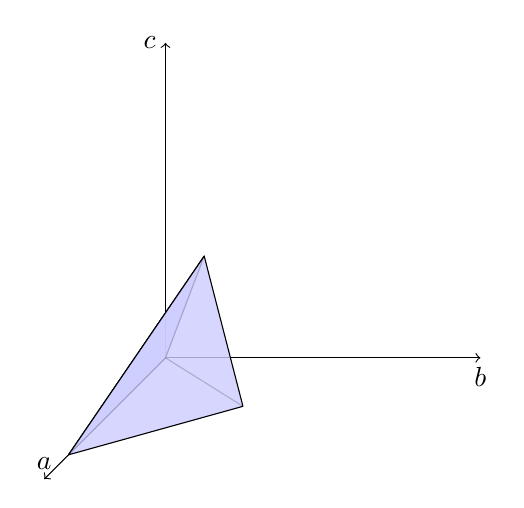
\begin{tikzpicture}[join=round,scale=0.8]
    \tikzstyle{conefill} = [fill=blue!20,fill opacity=0.8]
    \tikzstyle{ann} = [fill=white,font=\footnotesize,inner sep=1pt]
    \tikzstyle{ghostfill} = [fill=white]
    \tikzstyle{ghostdraw} = [draw=black!50]
    
    \draw[arrows=->,line width=.4pt](0,0,0)--(0,0,5); %Z_achse
    \draw[arrows=->,line width=.4pt](0,0,0)--(0,5,0); %Y-ACHSE
    \draw[arrows=->,line width=.4pt](0,0,0)--(5,0,0); %X-ACHSE
    %\draw[arrows=<-,line width=.4pt](.42,-.767)--(4,-2);
    
    \path (5,0,0) node[below] {$b$} (0,0,5) node[above] {$a$} (0,5,0) node[left] {$c$};
    
% letzte Koordinate ist A!!!
% zweite Koordinate ist C!!!
% dritte Koordinate ist B!!!
  
\filldraw[conefill](0,0,0)--(0,0,4)--(1,2,1)--cycle;
\filldraw[conefill](1,2,1)--(0,0,4)--(2,0,2)--cycle;
%\filldraw[conefill](1,2,1)--(0,0,0)--(2,0,2)--cycle;

\draw [opacity=0.2] (0,0,0) -- (2,0,2) ;
 
   
\end{tikzpicture}
        \caption{Gröbner cone for the first basis}
        \label{fig:singlegroebner}
    \end{subfigure}
    \begin{subfigure}[b]{0.48\linewidth}        %% or \columnwidth
        \centering
        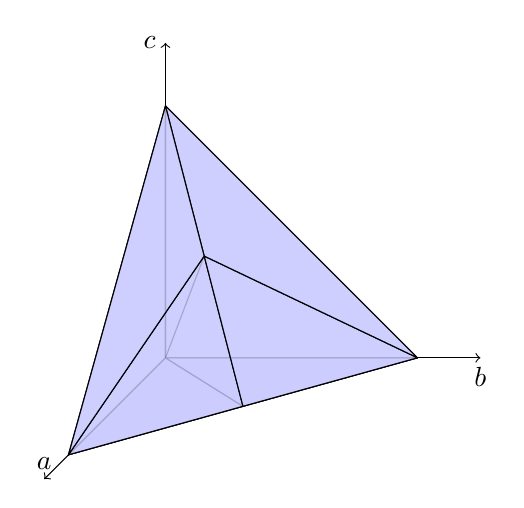
\begin{tikzpicture}[join=round,scale=0.8]
    \tikzstyle{conefill} = [fill=blue!20,fill opacity=0.8]
    \tikzstyle{ann} = [fill=white,font=\footnotesize,inner sep=1pt]
    \tikzstyle{ghostfill} = [fill=white]
    \tikzstyle{ghostdraw} = [draw=black!50]
    
    \draw[arrows=->,line width=.4pt](0,0,0)--(0,0,5); %Z_achse
    \draw[arrows=->,line width=.4pt](0,0,0)--(0,5,0); %Y-ACHSE
    \draw[arrows=->,line width=.4pt](0,0,0)--(5,0,0); %X-ACHSE
    %\draw[arrows=<-,line width=.4pt](.42,-.767)--(4,-2);
    
    \path (5,0,0) node[below] {$b$} (0,0,5) node[above] {$a$} (0,5,0) node[left] {$c$};
   
% erste Koordinate ist B!!! 
% zweite Koordinate ist C!!!   
% dritte Koordinate ist A!!!


% äußere Flächen!

\filldraw[conefill](0,0,0)--(0,4,0)--(0,0,4)--cycle;
\filldraw[conefill](0,0,0)--(4,0,0)--(0,0,4)--cycle;
\filldraw[conefill](0,0,0)--(4,0,0)--(0,4,0)--cycle;

% untenfläche
\filldraw[conefill](0,0,0)--(0,0,4)--(2,0,2)--cycle;
\filldraw[conefill](0,0,0)--(4,0,0)--(2,0,2)--cycle;

%
\filldraw[conefill](0,0,4)--(2,0,2)--(1,2,1)--cycle;
\filldraw[conefill](4,0,0)--(2,0,2)--(1,2,1)--cycle;

\filldraw[conefill](4,0,0)--(1,2,1)--(0,4,0)--cycle;
\filldraw[conefill](0,0,4)--(1,2,1)--(0,4,0)--cycle;

% zur Übersichtlichkeit die gerade im "inneren" des Cones
\draw [opacity=0.2] (0,0,0) -- (1,2,1) ;
\end{tikzpicture}
        \caption{Complete Gröbner fan}
        \label{fig:completegroebner}
    \end{subfigure}
    \caption{Gröbner fans for the given example}
    \label{fig:groebnerfans}
\end{figure}




Figure \ref{fig:singlegroebner} shows that the Gröbner fan is not complete, since the cone does not cover the whole positive orthant. In this example, the other reduced Gröbner basis can be obtained by applying the Buchberger-Algorithm with common monomial orders to the ideal $I$.
If the computed cones still do not cover the whole positive orthant, then further computations with weight vectors are necessary.
\begin{flushright}
$\lozenge$
\end{flushright} 
\end{env_example}

Example \ref{ex:groebnerfan} illustrates clearly that an arbitrary non-negative weight vector can be selected and if the vector lies in a certain cone, the corresponding Gröbner base will match with respect to this weight vector.  


This strategy is reasonable for small examples like above.
In genearal, the whole Gröbner fan can be computed with the Gröbner walk \cite{coxOshea}.\\
An inexpensive way to obtain all reduced Gröbner bases of a special ideal, the code ideal, will be explained in section \ref{subsec:enumerate}.

\newpage
\subsection{Toric Ideals}
\label{subsec:toric}
This work is focused on code ideals, so it is useful to define toric ideals first. Given a matrix $A =\left[a_{1},\dots, a_{n}  \right] \in \mathbb{Z}^{d \times n } $ and $u \in \mathbb{Z}^{n}$, which can be decomposed in $u^{+} $ and $u^{-}$, where $u^{+} $ and $u^{-}$ have non-negative coefficients and disjoint support, the toric ideals can be defined as follows.

\begin{env_definition}[Toric Ideal]
\cite{dueckjournal} A toric ideal $I_{A}$ is defined as
\begin{center}
$ \textbf{I}_{A} = \langle \textbf{x}^{u^{+}} - \textbf{x}^{u^{-}} \mid u \in ker \left(  A \right) \rangle . $
\end{center}


\end{env_definition}

The toric ideal can also be expressed as
\begin{center}
$ \textbf{I}_{A} =  \langle \textbf{x}^{u} - \textbf{x}^{v} \mid Au = Av,~ u,v \in \mathbb{N}^{n}_{0} \rangle .$
\end{center}

\newpage



 %mathematical background

\section{Enumerating Gröbner fans and Code Ideals}
\label{sec:enumerate}

Now that the mathematical background is given, the specific parts which are needed to implement the software and the connection between linear codes and Gröbner bases will be presented. The first section deals with enumerating all Gröbner bases with the help of breadth-first and reverse search followed by the degree compatible Gröbner bases.
After that, linear codes will be presented and to connect these two topics together, code ideals will be defined. 

\subsection{Enumerating Gröbner fans}
\label{subsec:enumerate}

In this section, two algorithms will be explained with the  purpose to enumerate the Gröbner fan.
To compute all Gröbner bases from a toric ideal $I_A$ , it is necessary to search the \textit{edge graph} of a Gröbner fan.\\
Two reduced Gröbner bases with respect to a term order covered by the generic weight vectors $c_{1}$, $c_{2}~$ are said to be adjacent if the two Gröbner cones share a common \textit{facet}. Given a reduced Gröbner basis with respect to the weight vector $c$, \textit{facet binomials} can be defined as follows.

\begin{env_definition}[Facet Binomial]
\cite{tigers}
The binomial $x^{\upalpha_{k}}-x^{\upbeta_k} \in \mathcal{G}_c~$, $\mathcal{G}_c~$is a reduced Gröbner basis with respect to the weight vector $c$, is a facet binomial of $\mathcal{G}_c$ if and only if there exists a vector $u \in \mathbb{R}^{n}$ which satisfies :

\begin{itemize}
\item
$ \lbrace \upalpha_{i} \cdot u > \upbeta_{i} \cdot u : i = 1, \dots , t, i \neq k \rbrace  
$
\item
$ \lbrace \upbeta_{k} \cdot u > \upalpha_{k} \cdot u \rbrace .$
\end{itemize}


\end{env_definition}
Computing the facet binomials of a reduced Gröbner basis $\mathcal{G}$ can be computationally expensive, because it is needed to solve as many linear programs as the cardinality of $\mathcal{G}$. Algorithm \ref{alg:facetsLP} for finding the facets can be as follows.

\newpage

\begin{algorithm}
\caption{Finding the facets of a reduced Gröbner bases of $I_A$ \cite{tigers}}
\label{alg:facetsLP}
\label{facets}
\begin{algorithmic}[1]

\Input
Reduced Gröbner basis $ \mathcal{G} = \lbrace \underline{x}^{a_{i}} - {x}^{b_{i}} : i = 1,\dots,t  \rbrace $ of $I_A$
\Output The facet binomials of $\mathcal{G}$
\State Facets := $\emptyset$

\For{\textbf{each} binomial $\underline{x}^{a_{i}} - {x}^{b_{i}}$ in $\mathcal{G}$}
\If{${a}_{i} - {b}_{i} \notin \textrm{cone generated by } \{{a}_{j} - {b}_{j} : \underline{x}^{a_{j}} - {x}^{b_{j}} \in \mathcal{G}, i \neq k \} $}
\State Facets := Facets $~\cup~\{{x}^{a_{i}} - {x}^{b_{i}} \} $
\EndIf

\EndFor \\
\Return Facets
%\EndProcedure
\end{algorithmic}
\end{algorithm}

%TODO Kleines Beispiel mit dem Simplexalgorithmus
\begin{env_example}\normalfont

% {a-e, b^2-1, b*d-e*f, b*e-d*f, b*f-d*e, c-e, d^2-1, d*e*f-b, e^2-1, f^2-1}
Given the reduced Gröbner basis \\
 $\mathcal{G} = \{x_1 - x_5,~x_{2}^{2}-1,~x_{2}x_{4}-x_{5}x_{6},~x_{2}x_{6}-x_{4}x_{5},~x_{3}-x_{5},~x_{4}^{2}-1,~x_{4}x_{5}x_{6}-x_{2},~x_{5}^{2}-1,~x_{6}^{2}-1  \}~$ and it shall be determined if the term $x_{2}x_{4}-x_{5}x_{6}~$ is a facet or not.
 With linear programming, it must be checked if the vector $b = {\left(0,1,0,1,-1,-1\right)}^{T}$ can be expressed by the matrix multiplication $A \cdot x = b~$, where \\
 \[
 A =
 \begin{pmatrix}
 1  & 0 & 0  & 0 & 0 & 0  & 0 & 0\\ 
 0  & 2 & 1  & 0 & 0 & -1 & 0 & 0\\  
 0  & 0 & 0  & 1 & 0 & 0  & 0 & 0\\ 
 0  & 0 & -1 & 0 & 2 & 1  & 0 & 0\\
 -1 & 0 & -1 & 1 & 0 & 1  & 2 & 0\\
 0  & 0 & 1  & 0 & 0 & 1  & 0 & 2
 \end{pmatrix} 
 .\] 
  
 Now the linear program can be set up to 
 \[
 	\begin{array}{lrcl}
 	\textrm{ }   & Ax    & =    & b   \\
 	\textrm{subject to}  & x     & \geq & 0
 			    
 	\end{array}
 \]
 

\begin{flushright}
$\lozenge$
\end{flushright}
\end{env_example}
\newpage 
Another way to find the facets without linear programming is possible with the property of the following leading ideals.

Let $\mathcal{G}_{c} $ be a reduced Gröbner basis with respect to a generic weight vector $c$. Then $x^{a} - x^{b}$ is a facet binomial of $\mathcal{G}_{c}$ only if $lt_{c}(I_{a})$ (see definition \ref{def:initial}) is the initial ideal of \[W_{a - b} = \langle x^{a}-x^{b}\rangle~+~ \langle x^{c}~|~x^{c}~\textrm{is a minimal generator of~} lt_{c}(I_{a}), x^{c} \neq x^{a} \rangle \] \cite{tigers}.
With the help of this property it is possible to define an algorithm to find a superset of facet binomials of a reduced Gröbner basis.

\begin{algorithm}
\caption{Finding a superset of the facet binomials
of a reduced Gröbner basis of $I_A$ \cite{tigers}}
\label{alg:facetSS}
\begin{algorithmic}[1]

\Input
Reduced Gröbner basis $ \mathcal{G}_{c} $ of $I_A$
\Output A superset SS of the facet binomial $\mathcal{G}_{c}$
\State SS := $\emptyset$
\For{\textbf{each} $x^{a} - x^{b} \in \mathcal{G}_{c}$}
\State $W_{a - b} := \langle x^{a}-x^{b}\rangle$
$~+~ \langle x^{c} \rangle$ \Comment{$x^{c}$ is defined as before}
\If{ $lt_{c}(I_{A})~$ is the leading ideal of $W_{a-b}$ with respect to $x_{a}>_{c}x_{b}$}
\State SS := SS $\cup~ \{x^{a}-x^{b} \}$

\EndIf
\EndFor \\
\Return SS

%\EndProcedure
\end{algorithmic}
\end{algorithm}
 

In the example \ref{ex:groebnerfan} the facet binomials of a Gröbner cone determine the border to an other Gröber cone.
In order to traverse from a Gröber base $\mathcal{G}_c$ to a neighboured Gröbner base $\mathcal{G}_{c'}$ with the certain facet $x^{\upalpha}-x^{\upbeta} $, a procedure making a local change from $\mathcal{G}_c$ to $\mathcal{G}_{c'}$ is required.
This procedure is called flip and is presented in algorithm \ref{alg:flip}. 
\newpage


\begin{algorithm}
\caption{Local change of reduced Gröbner bases in $I_A$ \cite{tigers}}
\label{alg:flip}
\begin{algorithmic}[1]

\Input
Reduced Gröbner basis $ \mathcal{G} $ of $I_A$

    A prescribed facet binomial $ \underline{x}^{a}_{i} - x^{b}_{i} \in \mathcal{G} $
%\Comment {The weight vector inducing $\mathcal{G}$ is generic and the leading terms are underlined}
\Output The reduced Gröbner basis is adjacent to $\mathcal{G}$ in which $ \underline{x}^{b}_{i} - x^{a}_{i} $ is a facet binomial.
\State Old 
$:= \lbrace \underline{x}^{a}_{i} - x^{b}_{i} \rbrace \cup
 \lbrace \underline{x}^{a}_{j} : \underline{x}^{a}_{j} - x^{b}_{j} \in \mathcal{G},
 j \neq i \rbrace $ \Comment{Prescribed Facet and leading terms only in Old }
 \State Temp $:= \lbrace \underline{x}^{b}_{i} - x^{a}_{i} \rbrace \cup 
 \lbrace \underline{x}^{a}_{j} : x^{a}_{j} \in Old  \rbrace $
 \Comment{Flipping the facet Binomial}
 \State New := Reduced Gröbner basis with respect to the new marking 
 \Comment{See algorithm \ref{alg:buchberger}.}
 \State $\mathcal{G}' = \left\lbrace \underline{x}^{b}_{i} - x^{a}_{i} \right\rbrace  $
 
 \For{\textbf{each} monomial h in New}
 \State Reduce $h$ with $\mathcal{G}$ to obtain the monomial $h'$.
 \State Add $h-h'$ to $\mathcal{G}'$ with $h$ marked as the leading term.
 \EndFor
 \State Auto-reduce $\mathcal{G}'$ to get $\mathcal{G}_{new}$
 \Comment{no term shall be divisible by a leading term}

%\EndProcedure
\end{algorithmic}
\end{algorithm}

This algorithm is correct and can terminate \cite{tigers}.
The main advantage of the algorithm is that no weight vectors must be stored or computed.
Weight vectors are carried implicitly and that is possible due to the binomial structure that this subroutine generates for every Gröbner basis. For this work \\ flip$({x}^{a}_{i} - x^{b}_{i},~\mathcal{G})$ means that algorithm \ref{alg:flip} is applied with the needed input.

\begin{env_example}\normalfont
Consider the reduced Gröbner basis with respect to a term order $\succ~$: $\mathcal{G}= \{x_{6}^{2}-1,~x_{5}^{2}-1,~x_{4}x_{5}x_{6} -x_{2},~x_{4}^{2}-1,~x_{3}-x_{5},~x_{2}x_{6}-x_{4}x_{5},~x_{2}x_{5}-x_{4}x_{6},~x_{2}x_{4}-x_{5}x_{6},~x_{2}^{2}-1,~x_{1}-x_{5}  \} $.

Applying the procedure flip$(x_{3}-x_{5}, \mathcal{G}$) leads to:

Old := $\{x_{3}-x_{5},~x_{6}^{2},~x_{5}^{2},~x_{4}x_{5}x_{6} ,~x_{4}^{2},~x_{2}x_{6},~x_{2}x_{5},~x_{2}x_{4},~x_{2}^{2},~x_{1} \} $ \\
Temp := $\{x_{5}-x_{3},~x_{6}^{2},~x_{5}^{2},~x_{4}x_{5}x_{6} ,~x_{4}^{2},~x_{2}x_{6},~x_{2}x_{5},~x_{2}x_{4},~x_{2}^{2},~x_{1} \} $

Now the new Gröbner basis has to be calculated, but first it useful to know that all pairs of binomials which have the least common multiple 1 will be auto-reduced to zero. In other words, it is only necessary to form the S-Pairs of binomials that are not relatively prime.

\begin{align*}
	S(x_{5}-x_{3},x_{5}^{2}) &= x_{3}x_{5} \\
	S(x_{5}-x_{3},x_{4}x_{5}x_{6}) &= x_{3}x_{4}x_{5} \\
	S(x_{5}-x_{3},x_{2}x_{5}) &= x_{2}x_{3} \\
	S(x_{5}-x_{3},x_{3}x_{5}) &= x_{3}^{2}
\end{align*}

Now the new Gröbner basis $\mathcal{G}'$ shall be filled with all monomials from $\mathcal{G}$.
The underlined terms are the terms reduced with $\mathcal{G}~$ and will be the new non-leading terms.
\begin{align*}
	x_{3}x_{5} &= x_{5}(x_{3}-x_{5}) + 1(x_{5}^{2}-1) &+ \underline{1} \\
	x_{3}x_{4}x_{6} &= x_{4}x_{6}(x_{3}-x_{5}) + 1(x_{4}x_{5}x_{6}-x_{2}) &+ \underline{x_{2}} \\
	x_{2}x_{3} &= x_{2}(x_{3}-x_{5}) + 1(x_{2}x_{5}- x_{4}x_{6}) &+ \underline{x_{4}x_{6}} \\
	x_{3}^{2} &= x_{3}(x_{3}-x_{5}) + x_{5}(x_{3}x_{5}) + 1(x_{5}^{2}-1)&+\underline{1} \\
	x_{1} &= (x_{1}-x_{5}) + (x_{5}-x_{3}) &+\underline{ x_{3}} \\
	x_{2}x_{6} &= (x_{2}x_{6}-x_{4}x_{5}) + x_{4}(x_{5}-x_{3}) &+\underline{ x_{3}x_{4}} \\
	x_{2}x_{4} &= (x_{2}x_{4}-x_{5}x_{6})+ x_{6}(x_{5}-x_{3}) &+\underline{x_{3}x_{6}}
\end{align*}

The other monomials of $\mathcal{G}~$ are not notated here because they did not get a new non-leading term.

This results to the Gröbner base : \\
$\mathcal{G}' = \{x_{5}-x_{3},~x_{6}^{2}-1,~x_{5}^{2}-1,~x_{4}x_{5}x_{6}-x_{2},~x_{4}^{2}-1,~ x_{2}x_{6}-x_{3}x_{4},~x_{2}x_{5}-x_{4}x_{6},~x_{2}x_{4}-x_{3}x_{6} ,~x_{2}^{2}-1,x_{1}-x_{3},~x_{3}x_{5}-1,~x_{3}x_{4}x_{6}-x_{2},~x_{2}x_{3}-x_{4}x_{6},~x_{3}^{2}-1 \}.$ \\
This Gröbner base is not reduced yet. After cancelling all binomials whose terms are divisible by some other leading terms the new reduced Gröbner basis is 
$\mathcal{G}_{new} = \{x_{5}-x_{3},~x_{6}^{2}-1,~x_{4}^{2}-1,~x_{2}x_{6}-x_{3}x_{4},~x_{2}x_{4}-x_{3}x_{6},~x_{2}^{2}-1,~x_{1}-x_{3},~x_{3}x_{4}x_{6}-x_{2},~x_{2}x_{3}-x_{4}x_{6},~x_{3}^{2}-1 \}.$

\begin{flushright}
$\lozenge$
\end{flushright}
\end{env_example}


\subsubsection{Breadth first search}

In this section an algorithm to enumerate the edge graph of a Gröbner fan via breath-first search and its drawbacks are presented.

\begin{algorithm}
\caption{Enumerating the edge graph of the Gröbner fan via breath-first search \cite{tigers}}
\label{alg:breath}
\begin{algorithmic}[1]

\Input
Any reduced Gröbner basis $ \mathcal{G}_0 $ of $I_A$
\Output All reduced Gröbner bases of $I_A$, (all vertices of the edge graph)
\State Todo := $\left[ \mathcal{G}_0 \right]  $
\State Verts := $\left[ \right] $
\While{Todo $\neq \emptyset$ }
\State $\mathcal{G}$ := first element in (Todo)
\State Remove $\mathcal{G} $ from Todo
\State add $\mathcal{G}$ to Verts 
\State determine list L of facet binomials of $\mathcal{G} $
\Comment{With linear programming}
 \For{\textbf{each} $x^{\upalpha}-x^{\upbeta} \in ~$ L  }
 \State $\mathcal{G}' =~$ flip($\mathcal{G},x^{\upalpha} - x^{\upbeta} $)
 \If{$\mathcal{G}' \notin \mathrm{Todo} \cup \mathrm{Verts}  $}
 \State add $\mathcal{G}'$ to Todo
 \EndIf
 \EndFor
\EndWhile 
\Return Verts

%\EndProcedure
\end{algorithmic}
\end{algorithm}

This algorithm is intuitive but has the drawback that every vertex of the edge graph must be stored and every vertex must be checked against all other vertices if it is a new vertex or not. 
The more vertices the edge graph has, the more expensive the calculation will be. Also the need of memory will arise if a Gröbner fan has a lot of cones.
 
 \newpage

\subsubsection{Reverse search tree}
The disadvantages can be canceled out with a memoryless algorithm, which runs linear depending on the size of output. The idea is to enumerate the edge graph with depth-first reverse search. The result will be a directed subgraph of the edge graph, called reverse search tree $T_{\succ}(I_{A}) $.\\
\begin{env_definition}[Mismarked Polynomial]
\cite{tigers}
A polynomial $f$ that has been marked with respect to the monomial order $>$  is mismarked with respect to the monomial order $>'$  .
\end{env_definition}

\begin{env_example}\normalfont
Consider the reduced Gröbner base \\ $\mathcal{G} = \left\lbrace x^{2}y-z,y^{2}-xz, zy-xy^{2}z \right\rbrace $ 
with a certain monomial order $>$, which is not the lexicograpic order.
Then, the second and last term are clearly mismarked with respect to $>_{lex}$.

Applying the flip-procedure $(\mathcal{G},y^{2}-xz)$ leads to the Gröbner base \\ $\mathcal{G} = \{x^{2}y-z,xz^{2}-y^{2}, zy-xy^{2}z \} $. Now only the last binomial is mismarked and using flip($\mathcal{G}$, $zy-xy^{2}z$) the result is the reduced Gröbner basis with respect to the lexicographic order $\mathcal{G} = \{xy^{2}z -xy,~xz^{2}-y^{2},~xy-z \} $. Note that every monomial can not be divided by the leading terms, so all Gröbner bases are reduced and no auto-reduce is necessary.
 
\begin{flushright}
$\lozenge$
\end{flushright} 
\end{env_example}


The \textit{reverse search tree} $T_{\succ}(I_{A}) $ with a given monomal order $ > $ can be defined as follows:
\begin{env_definition}[Reverse Search Tree]
\label{def:reverse}
\cite{tigers} For two reduced Gröbner bases $\mathcal{G}_{i}$ and $\mathcal{G}_{j}~$, $[\mathcal{G}_{i},\mathcal{G}_{j} ]~$ directed from $\mathcal{G}_{i}~$to $\mathcal{G}_{j}~$ is an edge of $~T_{\succ}(I_{A}) $ if $\mathcal{G}_{i}$ is obtained from $\mathcal{G}_{j}$ by the algorithm \ref{alg:flip} flip$(x^{\upalpha} - x^{\upbeta},~\mathcal{G}_{i}).$ $x^{\upalpha}$ is lexicographically maximal among all facet binomials of $\mathcal{G}_{i}$, that are mismarked with respect to $>$.
\end{env_definition}


\newpage

It can be shown that the reverse search tree is an acyclic graph with a unique sink and from any reduced Gröbner basis of $\mathcal{G}_{c} $ of a toric ideal $I_{A}$, there is a unique path to the sink $\mathcal{G}_{>}$ \cite{tigers} .
Unlike the Gröbner walk procedure, there are still no weight vectors involved, but in return every facet of the Gröebner cone must be computed, which can be computionally expensive for reduced Gröbner basis with many polynomials.

\begin{algorithm}
\caption{Enumerating the edge graph of the Gröbner fan via reverse search \cite{tigers}}
\label{alg:reverse}
\begin{algorithmic}[1]

\Input
Any reduced Gröbner basis $ \mathcal{R}_{>} $ of $I_A$ and its term order $>$
\Output All reduced Gröbner bases of $I_A$, (all vertices of the edge graph)
\State $\mathcal{G} := \mathcal{R}_{>}$;$~j := 0$;$~L := $ list of facet binomials of $\mathcal{G}$ marked by $>$
\State add $\mathcal{G}$ to output
\Repeat
\While{ $ j < \left|L\right| $ }

\State j := j + 1
\State $\mathcal{G}':= $ flip($\mathcal{G}$,$L[j]$);

\If{ $[\mathcal{G}',\mathcal{G}] \in T_{>}(I_{A}) $ }
\Comment{ Check for adjacency }
\State $\mathcal{G} := \mathcal{G}' $;   $~j := 0$
\State $ L := $ list of facet of $\mathcal{G}$ marked by $>$
\State add $ \mathcal{G}$ to output

\EndIf 

\EndWhile

\If{$ \mathcal{G} \neq \mathcal{R}_{>}$}
\State $\mathcal{G}' :=~$ unique element such that $[\mathcal{G}',\mathcal{G}] \in T_{>}(I_{A}) $
\State $j := 0$
\State $L := $ list of facets of $\mathcal{G}'$ marked by $>$

\Repeat
\State $j := j + 1$
\Until{the common facet of $\mathcal{G}$ and $\mathcal{G}'$ is the $j$-th facet of $L$ }

\EndIf

\Until{$\mathcal{G} = \mathcal{R}_{>}$ and $ j = \left|L\right| $ }


%\EndProcedure
\end{algorithmic}
\end{algorithm}

\newpage

\begin{env_example}\normalfont
Consider the ideal with the reduced Gröbner basis with respect to the lexicographic order $x_{1} > \ldots > x_{6} $
\[ \mathcal{G} = \{x_{1} - x_{2}, x_{3} - x_{4}, x_{5}-x_{6} , x_{2}^{2} -1 , x_{4}^{2} - 1, x_{6}^{2} - 1 \}. \]

Applying the breath-first search algorithm for this reduced Gröbner basis results to the following edge graph.\\
Using the reverse search method, this search tree on figure \ref{fig:reverse} results.


\begin{figure}[h]
    \centering
    \begin{subfigure}[b]{0.48\linewidth}        %% or \columnwidth
        \centering
        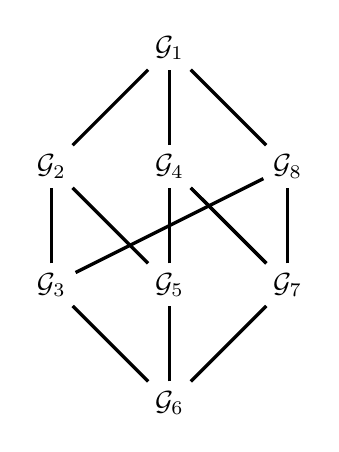
\begin{tikzpicture}[scale = 0.5]
\node (A) at (0,0) {$\mathcal{G}_{1}$};

\node (C) at (-3,-3) {$\mathcal{G}_{2}$};
\node (D) at (0,-3) {$\mathcal{G}_{4}$};
\node (B) at (3,-3) {$\mathcal{G}_{8}$};

\node (E) at (3,-6) {$\mathcal{G}_{7}$};
\node (F) at (-3,-6) {$\mathcal{G}_{3}$};
\node (G) at (0,-6) {$\mathcal{G}_{5}$};

\node (H) at (0,-9) {$\mathcal{G}_{6}$};


\draw[-, very thick] (D) to (A);
\draw[-, very thick] (C) to (A);
\draw[-, very thick] (B) to (A);

\draw[-, very thick] (E) to (D);
\draw[-, very thick] (F) to (C);
\draw[-, very thick] (G) to (D);
\draw[-, very thick] (G) to (C);
\draw[-, very thick] (E) to (D);
\draw[-, very thick] (F) to (B);
\draw[-, very thick] (E) to (B);

\draw[-, very thick] (H) to (G);
\draw[-, very thick] (H) to (F);
\draw[-, very thick] (H) to (E);
%\draw[-, very thick] (F) to (G);

\end{tikzpicture}
        \caption{Complete edge graph}
        \label{fig:breadth}
    \end{subfigure}
    \begin{subfigure}[b]{0.48\linewidth}        %% or \columnwidth
        \centering
        
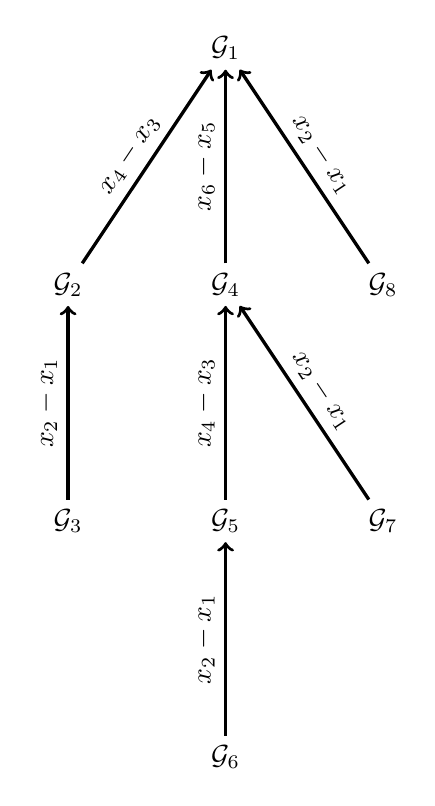
\begin{tikzpicture}

\node (A) at (0,0) {$\mathcal{G}_{1}$};

\node (C) at (-2,-3) {$\mathcal{G}_{2}$};
\node (D) at (0,-3) {$\mathcal{G}_{4}$};
\node (B) at (2,-3) {$\mathcal{G}_{8}$};

\node (E) at (2,-6) {$\mathcal{G}_{7}$};
\node (F) at (-2,-6) {$\mathcal{G}_{3}$};
\node (G) at (0,-6) {$\mathcal{G}_{5}$};

\node (H) at (0,-9) {$\mathcal{G}_{6}$};


\draw[->, very thick] (D) to node[midway, above, sloped]  {$x_{6}-x_{5}$}(A);
\draw[->, very thick] (C) to node[midway, above, sloped]   {$x_{4}-x_{3}$} (A);
\draw[->, very thick] (B) to node[midway, above, sloped]   {$x_{2}-x_{1}$} (A);

\draw[->, very thick] (E) to node[midway, above, sloped]   {$x_{2}-x_{1}$} (D);
\draw[->, very thick] (F) to node[midway, above, sloped]   {$x_{2}-x_{1}$}(C);
\draw[->, very thick] (G) to node[midway, above, sloped]   {$x_{4}-x_{3}$}(D);

\draw[->, very thick] (H) to node[midway, above, sloped]   {$x_{2}-x_{1}$}(G);


\end{tikzpicture}

        \caption{Reverse search tree}
        \label{fig:reverse}
    \end{subfigure}
    \caption{Comparison between the breath-first search and the reverse search}
    \label{fig:graph}
\end{figure}
\newpage
%thx to http://www.math.tugraz.at/~huss/new/teaching/computermathematik09/dateien/tikz_demonstration.pdf
The flipping binomials at figure \ref{fig:reverse} are written on the edges.

The Gröbner bases are:
\begin{center}
$\mathcal{G}_{1} = \{x_{1}-x_{2},x_{3}-x_{4},x_{5}-x_{6},x_{2}^{2}-1,x_{4}^{2}-1,x_{6}^{2}-1 \} $ \\
$\mathcal{G}_{2} = \{x_{1}-x_{2},x_{4}-x_{3},x_{5}-x_{6},x_{2}^{2}-1,x_{3}^{2}-1,x_{6}^{2}-1 \} $ \\
$\mathcal{G}_{3} = \{x_{2}-x_{1},x_{4}-x_{3},x_{5}-x_{6},x_{1}^{2}-1,x_{3}^{2}-1,x_{6}^{2}-1 \} $ \\
$\mathcal{G}_{4} = \{x_{1}-x_{2},x_{3}-x_{4},x_{6}-x_{5},x_{2}^{2}-1,x_{4}^{2}-1,x_{5}^{2}-1 \} $ \\
$\mathcal{G}_{5} = \{x_{1}-x_{2},x_{4}-x_{3},x_{6}-x_{5},x_{2}^{2}-1,x_{3}^{2}-1,x_{5}^{2}-1 \} $ \\
$\mathcal{G}_{6} = \{x_{2}-x_{1},x_{4}-x_{3},x_{6}-x_{5},x_{1}^{2}-1,x_{3}^{2}-1,x_{5}^{2}-1 \} $ \\
$\mathcal{G}_{7} = \{x_{2}-x_{1},x_{3}-x_{4},x_{6}-x_{5},x_{1}^{2}-1,x_{4}^{2}-1,x_{5}^{2}-1 \} $ \\
$\mathcal{G}_{8} = \{x_{2}-x_{1},x_{3}-x_{4},x_{5}-x_{6},x_{1}^{2}-1,x_{4}^{2}-1,x_{6}^{2}-1 \} $ \\
\end{center}

A lot of edges were saved which results to less computation.
\begin{flushright}
$\lozenge$
\end{flushright}
\end{env_example}




\subsection{Degree compatible Gröbner basis}
\label{subsec:degreecomp}
Computing the whole Gröbner fan can be very expensive and not every Gröbner basis is interesting.
In this section, the degree compatible Gröbner fan is introduced and how the algorithm can
be changed so that only the degree compatible Gröbner fan will be computed.\\
\begin{env_definition}[Degree compatible Gröbner basis]
\cite{dueckpaper}
A reduced \\ Gröbner basis for an ideal I with respect to a certain monomial order is
degree compatible if and only if the corresponding Gröbner cone contains the all-one vector \textbf{1}.
\end{env_definition}
Equivalent to this, the leading term of every polynomial must have the highest degree.
Since a Gröbner fan is homogeneous at $\mathbb{R}^{n}_{+}$, there will be at least one degree compatible Gröbner basis.
That is a special case can be easily determined as follows.

\begin{env_definition}[Only degree compatible Gröbner basis]
\cite{dueckpaper}
A Gröbner basis $\mathcal{G}$ with respect to a degree compatible monomial ordering $>$  is the only degree compatible Gröbner basis for an ideal if and only if
\[ deg(x^{a}) > deg(x^{b})~~ \forall~~ x^{a}-x^{b}\in \mathcal{G}. \] 
\end{env_definition}

This can be also described by the all-one vector that lies completely in a Gröbner cone of a Gröbner basis $\mathcal{G}$.
It follows that the all-one vector does not intersect with any facets if there is only one degree compatible Gröbner basis. \\

The algorithms \ref{alg:breath} and \ref{alg:reverse} can be adapted in order to compute only the degree compatible Gröbner fan.\\ 
The breadth-first search now needs a degree compatible Gröbner basis as an input. This can be achieved by applying the Buchberger Algorithm with a degree compatible monomial, for example the \textit{grlex} order. After that it is required that the Gröbner basis is checked if its is the only degree compatible basis. %see only degree compatible Gröbner basis
Also the only facet binomials $x^{a} - x^{b}$ which are allowed to be "flipped" are the binomials that satisfy the condition
deg(x$^{a}$) = deg(x$^{b}$). \\ \\
The reverse search tree can be deployed as in definition \ref{def:reverse} but with the restriction that deg(x$^{a}$) = deg(x$^{b}$) must be satisfied to traverse the degree compatible Gröbner fan.
It can be ensured by \cite{dueckpaper} that at least one such facet binomial will be found. 
The sink of the reverse search tree contains binomials that are not mismarked with respect to some degree compatible monomial order. 

   

\newpage

\subsection{Linear Codes over Prime Fields}
\label{subsec:linearcodes}
This work is focused on computing the Gröbner fan of linear codes. Now the mathematic background of the Gröbner fans is given, the linear Codes and code ideals have to be defined to give a connection between these two topics.\\ 
Let $\mathbb{F}$ be a finite field and let $n~$and $k\in \mathbb{N}~$ with $n\geq k$.
\begin{env_definition}[Linear Code]
\cite{dueckjournal} A linear code of length n and dimension k over $\mathbb{F}~$is the image $\mathcal{C}~$of a injective linear mapping $\phi~:~\mathbb{F}^{k} \rightarrow \mathbb{F}^{n}.$
\end{env_definition} 
Such a code will be denoted as an [$n,k$] code and its elements are called codewords. The codewords are written 
as row vectors. The Code $\mathcal{C}~$can alternatively be described as a row space matrix of $G \in \mathbb{F}^{k \times n}$. The rows of $G$ form a basis of $\mathcal{C}$.
The matrix $G$ is also called \textit{generator matrix} for $\mathcal{C}$.
\begin{env_definition}[Standard form]
\cite{dueckjournal}
A $[n,k]~$ code $\mathcal{C}~$is in standard form if it has a generator matrix like $G = (I_{k}| M)$, where $I_{k}$ is the $k \times k$ matrix.
\end{env_definition}


\begin{env_example}\normalfont
Consider the binary $[7,4]$ Hamming Code with its generator matrix

\[
G =
\begin{pmatrix}
1 & 0 & 0 & 0 & 1 & 1 & 0 \\ 
0 & 1 & 0 & 0 & 1 & 0 & 1 \\  
0 & 0 & 1 & 0 & 1 & 1 & 1 \\ 
0 & 0 & 0 & 1 & 0 & 1 & 1
\end{pmatrix} 
.\]

The codeword $c~$of the word $x~$is obtained with the vector-multiplication
\[
     xG = c. \\
 \]
 Let $x$ be $\left(1,0,1,0\right)$, then the codeword c results to:
 \[
      \left(1,0,1,0\right) \cdot \begin{pmatrix}
      1 & 0 & 0 & 0 & 1 & 1 & 0 \\ 
      0 & 1 & 0 & 0 & 1 & 0 & 1 \\  
      0 & 0 & 1 & 0 & 1 & 1 & 1 \\ 
      0 & 0 & 0 & 1 & 0 & 1 & 1
      \end{pmatrix}   = \left(1,0,1,0,0,0,1\right) \\
  \]
\begin{flushright}
$\lozenge$
\end{flushright} 

\end{env_example}

Two codes are equivalent if one generator matrix can be obtained from the other by permuting columns and rows.
It follows that every linear code is equivalent to a linear code in standard form \cite{dueckjournal}. \\

A linear Code $\mathcal{C}$ can be \textit{punctured} by deleting individual code symbols.
This reduces the length of the code and rises the data rate for a transmission of a code.


\subsection{Code Ideals}
\label{subsec:codeideals}
In this section, the linear codes and the Gröbner bases come together.\\
Each linear code $\mathcal{C}~$ can be associated to a binomial ideal \cite{dueckpaper}. Let $\mathcal{C}~$ be a $[n,k]$ code and let 
$\mathbb{K}[\textbf{x}]=\mathbb{K}[x_{1},\dots,x_{n}]$.
Then the \textit{code ideal} can be defined as follows:

\begin{env_definition}[Code Ideal]
\cite{dueckpaper} A code ideal $I(\mathcal{C})$ is the union between the toric ideal and a nonprime ideal $I_{p}$, such that
\begin{align*}
 I_{\mathcal{C}} & = \langle \textbf{x}^{c} - \textbf{x}^{c'} | c - c' \in \mathcal{C}  \rangle + I_{p},\\
\textrm{where} ~ I_{p} & = \langle x_{i}^{p} - 1 | 1 \leq i \leq n \rangle .
\end{align*}
\end{env_definition}

\newpage

\begin{env_example} \normalfont
 Let $\mathcal{C}_{1}~$ be a binary $[6,3]$ code with generator matrix
\[
G_{1} =
\begin{pmatrix}
1 & 0 & 0 & 0 & 1 & 0 \\ 
0 & 1 & 0 & 1 & 1 & 1 \\  
0 & 0 & 1 & 0 & 1 & 0  
\end{pmatrix} 
.\]

The associated code ideal $I(\mathcal{C})$ leads to: \newline
\begin{align*}
I(\mathcal{C}) = &\{x_{1}-x_{5},~x_{2}-x_{4}x_{5}x_{6},~x_{3}-x_{5}  \} ~\cup \\ &\{x_{1}^{2}-1,~x_{2}^{2}-1,~x_{3}^{2}-1,~x_{4}^{2}-1,~x_{5}^{2}-1,~x_{6}^{2}-1\}
\end{align*}
Note that the terms $x_{1}^{2}-1,~x_{2}^{2}-1,~x_{3}^{2}-1 $ are divisible by the leading terms of the toric ideal.
The reduced Gröbner basis $\mathcal{G}_{>}$ with respect to the lexicographic ordering $>$ with $x_{1} > \cdots > x_{6}$ is:
\begin{center}
$ \mathcal{G}_{>} = \{x_{1}-x_{5},~x_{2}-x_{4}x_{5}x_{6},~x_{3}-x_{5}  \} \cup \{x_{4}^{2}-1,~x_{5}^{2}-1,~x_{6}^{2}-1  \}  $
\end{center}

Puncturing the fourth symbol $x_4$ results to new reduced Gröbner base 
\begin{center}
$ \mathcal{G}_{>} = \{x_{1}-x_{5},~x_{2}-x_{5}x_{6},~x_{3}-x_{5}  \} \cup \{x_{5}^{2}-1,~x_{6}^{2}-1  \}  $.
\end{center}
Note that the term $x_{4}^{2}-1~$was auto-reduced.


\begin{flushright}
$\lozenge$
\end{flushright} 

\end{env_example}

 

\newpage %enumerating gröbner and linear codes
% this file is drba_sw.tex
\section{Software}
\label{sec:software}
This section is all about the practical part of this work. At first, a brief reason why the software is implemented in C is given. Secondly, an accurate description is presented of how the software can be compiled and used for own demand.
After that, the software is tested on some randomly generated linear Codes. The number of degree compatible and all Groebner bases are presented and comparision of the operational time agains Gfan$[Gfan]$ is presented.  \\ \newline
This software is a re-implementation of TiGERS $[Tigers]$. All features that are needed for the code ideals were added, also the adapted algorithms for computing degree compatible Groebner bases with reverse search and breath-first search were implemented.   
Additional features are explained later in Section \ref{subsec:manual}.
The programming language of choice is C because it is fast and the capability to make own data structures are simple and sufficient enough.







\subsection{Data Structures}
\label{subsec:datastructure}
With the special attribute that code ideals only contains binomials and monomials can be represented as an exponent vector, it is useful to store this vector in to dynamic array.

\lstset{language=C, commentstyle=\color{green}, backgroundcolor=\color{white}, keywordstyle=\color{blue}, 
basicstyle = \ttfamily \color{black} \footnotesize , 
caption = {Data structure of binomials[Tigers]}, } 
\begin{lstlisting} 
typedef struct bin_tag *binomial;
struct bin_tag{
    int *exps1;
    int *exps2;
    int *E;
    int ff;
    int bf;
    binomial next;
};

\end{lstlisting}

The pointer \emph{exps1} stores the exponent vector of the first monomial and \emph{exps2} does it with the second monomial.
The integer ff is a flag which shows if binomial is a facet binomial or not and bf tells if there is a monomial or binomial.
The pointer binomial next indicates that binomials are linked together like a linear list, which is necessary to describe ideals and Groebner bases.\\

The next code snippet shows the other important data structure. Again, it is a linked list like the binomials with the purpose to connect all reduced Groebner together, which is needed for the breath-first search.\\

The first four integers show off the identification number of the vertex of the edge graph, the number of facet binomials, number of binomials and the highest degree. Next is a pointer to the next generating set of the linked list.
 

\lstset{language=C, commentstyle=\color{green}, backgroundcolor=\color{white}, keywordstyle=\color{blue}, 
basicstyle = \ttfamily \color{black} \footnotesize , 
caption = {Data structure of generating sets [Tigers]}, } 
\begin{lstlisting} 
typedef struct gset_tag *gset;

/* Linked List of gset_tag which contiains the binomial and the
   caching informations*/
struct gset_tag{
    int id;
    int nfacets;
    int nelts;
    int deg;
    binomial bottom;
    binomial cache_edge;
    struct gset_tag *cache_vtx;
    struct gset_tag *next;
};

\end{lstlisting}

 


 


\subsection{Manual}
\label{subsec:manual}
This software was programmed and evaluated with Linux, so at first, it is needed to compile the software. The makefile is given and it only takes the console, moving to the direction where folder is and typing 'make'. \\
All inputs, outputs, options and flags are passed with the commandline arguments. At first it is useful to run the program with the purpose to print the help-message only with the command
\texttt{./cidgel -h}.

\lstset{basicstyle=\footnotesize, columns=fullflexible,showspaces=false,breakatwhitespace=true,caption = {Code Snippet of the help-message}} 
\begin{lstlisting} 

static char *helpmsg[] = {
    "Function: Enumerate all or d.c Groebner bases of a code ideal I(C).",
    "          \n",
    "Options:\n",
    "    -h            print this message\n"
    "    -i (filename) set file name for input  [default: stdin]\n",
    "    -o (filename) set file name for output [default: stdout]\n",
    "    -m (filename) set file name for code-matching \n",
    "    -R            only compute root of tree \n",
    "    -r            compute all grobner bases [done by default]\n",
    "    -C            turn partial caching on   [done by default]\n",
    "    -c            turn partial caching off \n",
    "    -T            print edges of search tree \n",
    "    -t            do not print edges of search tree [assumed by default]\n",  
    "    -L            print vertices by giving initial ideals\n",
    "                     and printing facet biomials.\n",
    "    -l            print vertices as grobner bases   [done by default]\n",
    "    -F            Use only linear algebra when testing facets [default]\n",
    "    -f            use FLIPPABILITY test first when determining facets\n",
    "    -e            use exhaustive search instead of reverse search\n",
    "    -E            use reverse search                   [default]\n",
    "    -d            degree compatible Groebner bases only         \n",
    "    -n            do not print vertices or edges                \n",
    "    -p            calculate Groebner fans of punctured codes    \n",
    NULL
};

\end{lstlisting}

The listing above shows all options that are available. These flags can be passed in arbitrary order to the program. An example will be shown next.
But before it is necessary to write a matrix and storing it into a file.

For example, the data has the name '\texttt{matrix}', has the following content and is in the same folder as the compiled software.
\lstset{caption = {Example-input}}
\begin{lstlisting}
M: { 6 10 2 :
1 0 0 0 0 0 0 0 1 1 
0 1 0 0 0 0 1 1 0 0 
0 0 1 0 0 0 1 1 1 1 
0 0 0 1 0 0 0 1 1 1 
0 0 0 0 1 0 1 0 0 0 
0 0 0 0 0 1 0 1 0 1 
}
\end{lstlisting}

This Matrix is a generator matrix for a binary $[10,6]$ code in essential standard form. 
The first number in the first row gives the code dimension, the second tells the length of the codeword and the last number indicates in which primary field the generator matrix shall be evaluated.\\

Now if the degree compatible Groebner bases of this generator  matrix without printing the Groebner basis shall be written in a outputfile called \texttt{Example-output}. Additionally the linear programming shall be leaved out, then the program call is: \texttt{./cidgel -i Example-input -o Example-output -d -n -f}.
The user do not has to specify an output file, the result will be printed in the console then.


\lstset{caption = {Snipped of the example outsput}}
\begin{lstlisting}
% starting GB:
F: 2
R: 10
G: {a-i*j, b-g*h, c-g*h*i*j, d-h*i*j, e-g, f-h*j, g^2-1, h^2-1, i^2-1, j^2-1}

 Enumerating degree compatible Groebner bases
   using reverse search
   taking input from randomgenerator/10_6
   with partial caching
   using wall ideal pretest for facet checking

Number of Groebner bases found 216
Number of edges of state polytope 792
max caching depth      10
max facet binomials    18
min facet binomials    12
max binomials in GB    41
min binomials in GB    40
max degree             3
min degree             2
randomgenerator/10_6: Reverse Search,   Caching,  A-pretest,
time used (in seconds) 42.16
\end{lstlisting}
  






\subsection{Computational experience}
\label{subsec:compexp} 
In this section the difference between degree compatible Groebner bases and all Groebner bases from a linear Code are researched. Furthermore, the time for all Grooebner bases is compared against Gfan.

%TODO: HIER EIN PAAR BILDER HOCHLADEN
%TODO: EXTREMBEISPIEL ZEIGEN UND VLLT SAGEN WARUM NICHT FÜR GRÖSSERE BASEN 



\subsection{Documentation and electronic availability}
\label{subsec:docu}
A HTML-based documentation of the software is created with the help of doxygen.$[doxygen]$

\newpage

 %software
% this file is drba_tp.tex
% title page
\section{Future Work}
Even if the algorithms are well suited for the given problems, this software can be improved.
The algorithms themselves may already have mathematically the best performance. 
Section \ref{subsec:compexp} shows that the computation of facets is the most expensive step, so the performance can be heavily improved by enhancing the linear programming.
The software uses a built-in LP solver mentioned in \cite{tigers}, but extern LP-solver like the GLPK (GNU Linear Programming Kit) could be more efficient. \\
The software package CaTS \cite{cats} enumerates all reduced Gröbner bases for a lattice Ideal. CaTS uses an external LP-Solver too to improve the performance.
\\\\
Another approach will be parallelization of the computation of facets. To compute the facets, a certain amount of linear programs have to be set up, which can be solved independently. Every processor core of the computing unit can solve the linear programs.\\
If a LP solver is thread-safe, both ideas can be put together and lead to a large speedup. 

\newpage%future work
% this file is drba_tp.tex
% title page
\section{Conclusion}

In this thesis a software was introduced to compute the Gröbner fan of linear codes. Firstly, the mathematical background and concepts were discussed with the purpose to develop the software, with the hope that it might be useful for researches and other thesis that only needs the degree compatible Gröbner fan.\\
\\~
In my knowledge, no other software provides this useful feature to compute the degree compatible Gröbner fan. Computing the degree compatible can be dramatically faster than computing the whole Gröbner fan.\\
\\~
Programming in C was a pleasure. The given data structures and the well written algorithms from TiGERS \cite{tigers} made it easy to extend the software with a lot of new features in terms of linear codes and the degree compatible Gröbner fan.  %conclusions 
\newpage
\renewcommand{\refname}{Bibliography}
\bibliography{literatur}





\end{document}